\section{Comparaison des deux méthodes}

\subsection{Différences entre NMF et K-means}

Contrairement à la NMF, qui attribue à chaque segment un poids pour chacun des topics, K-means attribue chaque segment à un seul cluster. Cette différence est importante : la NMF autorise une lecture plus graduelle des thèmes, tandis que K-means produit une classification plus nette. Un segment appartient à un cluster principal, même s'il peut contenir plusieurs motifs thématiques.

La NMF permet donc d'observer la présence simultanée de plusieurs thèmes dans un même segment, alors que K-means propose une lecture plus catégorielle du corpus. Les deux méthodes ne répondent donc pas exactement au même objectif : la première met en évidence des topics latents, tandis que la seconde regroupe les segments selon leur proximité lexicale.

\subsection{Convergences thématiques}

Les intitulés obtenus montrent que les clusters couvrent des dimensions proches de celles observées avec la NMF. On retrouve par exemple des ensembles liés au travail, à la mine, à la finance, à la religion, à la famille, au monde domestique, à la guerre ou encore aux espaces urbains. Cette convergence entre les deux méthodes est intéressante, car elle indique que certains thèmes apparaissent de manière stable dans le corpus, indépendamment de la méthode utilisée.

\begin{figure}[H]
    \centering
    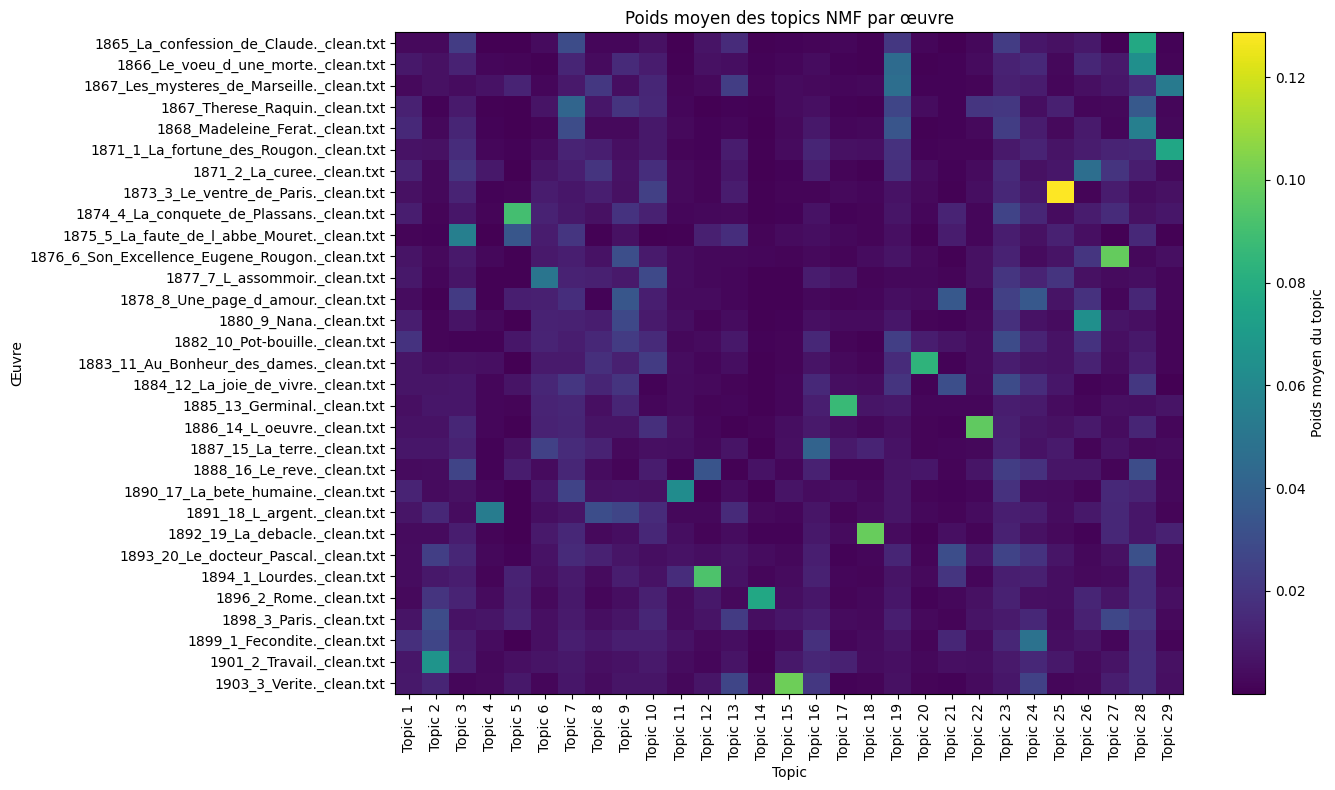
\includegraphics[width=\textwidth]{figure/headmap_nmf.png}
    \caption{Heatmap des poids des mots dans les topics NMF}
    \label{fig:heatmap_nmf}
\end{figure}
    
\begin{figure}[H]
    \centering
    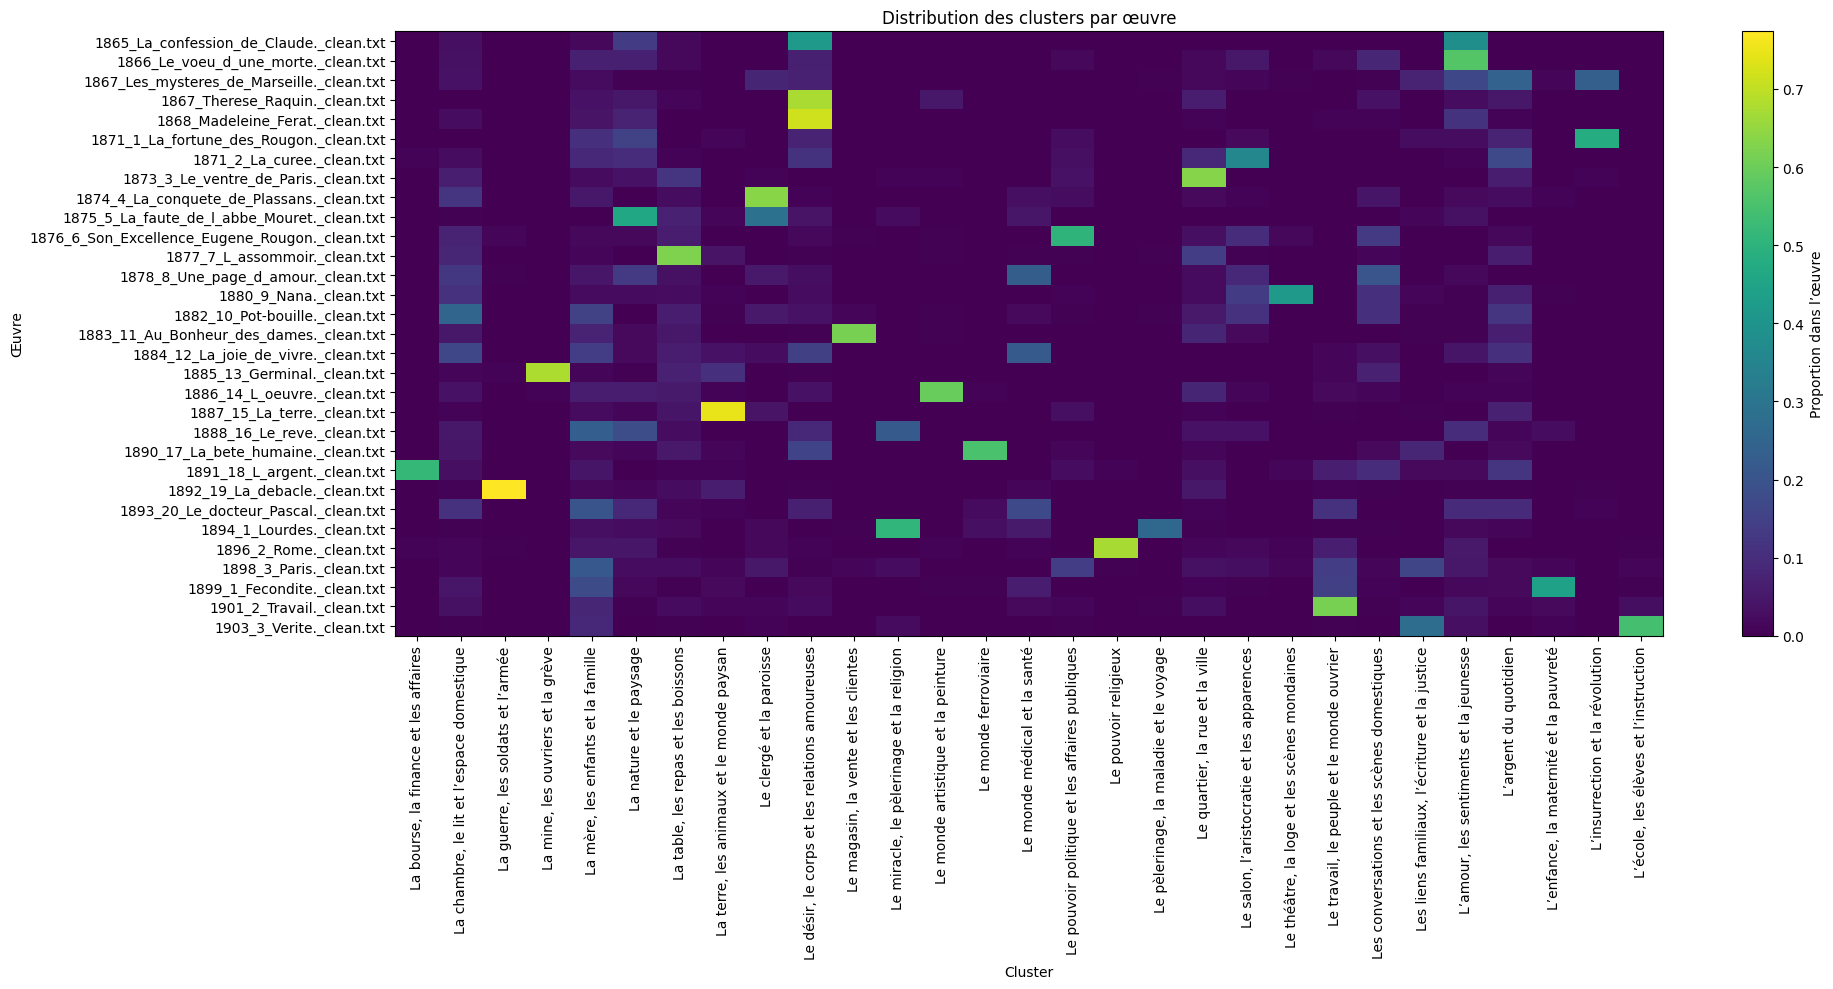
\includegraphics[width=\textwidth]{figure/headmap_kmeans.png}
    \caption{Heatmap des poids des mots dans les clusters K-means}
    \label{fig:heatmap_kmeans}
\end{figure}

La méthode K-means permet ainsi de compléter l'analyse réalisée avec la NMF. Elle offre une autre manière d'observer les régularités thématiques du corpus, non plus sous la forme de topics latents, mais sous la forme de groupes de segments lexicalement proches. Cette approche confirme plusieurs motifs déjà observés avec la NMF, notamment autour du travail, de la religion, de la famille, de l'argent, de la guerre, de la mine, du commerce ou de l'espace domestique.

\subsection{Distribution des thèmes par œuvre}

Afin d'observer la présence des clusters dans chaque roman, une table croisée a été construite entre les fichiers du corpus et les clusters thématiques. La normalisation par ligne permet d'obtenir, pour chaque œuvre, la proportion de segments associés à chaque cluster.

Cette analyse est importante, car elle permet de relier les clusters aux romans. Certains clusters peuvent être très transversaux et apparaître dans de nombreuses œuvres, tandis que d'autres peuvent être fortement associés à un roman précis. Par exemple, un cluster lié à la mine peut être particulièrement représenté dans \textit{Germinal}, tandis qu'un cluster lié à la finance peut être plus présent dans \textit{L'Argent}. De la même manière, les clusters associés au commerce peuvent être importants dans \textit{Au Bonheur des dames}, et ceux liés à la guerre dans \textit{La Débâcle}.

Une analyse similaire a été réalisée au niveau des grandes familles de motifs. Cette seconde visualisation offre une lecture plus synthétique. Elle permet de comparer les romans selon les grandes familles de motifs qui les structurent. Cette approche est particulièrement utile pour repérer des oppositions ou des proximités entre les œuvres : certains romans peuvent être dominés par des motifs de vie quotidienne, tandis que d'autres accordent plus de place aux institutions, à la religion, à la guerre ou aux conflits sociaux.

\subsection{Apport de la double approche}

Ainsi, K-means ne remplace pas la NMF, mais il constitue un complément méthodologique utile. En croisant les résultats des deux méthodes, il devient possible de distinguer les thèmes particulièrement stables de ceux qui dépendent davantage du modèle utilisé. Cette double approche renforce donc la solidité de l'analyse, tout en conservant une part d'interprétation qualitative indispensable dans l'étude d'un corpus littéraire.